\section{Руководство по использованию программного средства}
\label{sec:manual}

В данном разделе приведены основные сведения по работе с программным средством.

Приложение данного дипломного проекта (а точнее, его клиентская часть) не требует установки и настройки на
конечных устройствах пользователя, поскольку представляет собой веб-приложение. Как и было заявлено в требованиях,
для корректной работы программного средства необходим один из следующих браузеров с соответствующей минимальной версией:

\begin{itemize}
	\item Google Chrome 70;
	\item Opera 58;
	\item Mozilla Firefox 66;
	\item Apple Safari 12.0;
	\item Microsoft Edge 44.
\end{itemize}

Далее рассмотрены основные функции, предоставляемые приложением пользователям.

После авторизации открывается главная страница приложения, представленная на рисунке~\ref{fig:manual:agenda_screen}.
Весь профиль заполняется с помощью формы на 4 страницы. Результат после заполнения каждой страницы сохраняется.

\begin{figure}[ht]
  \centering
    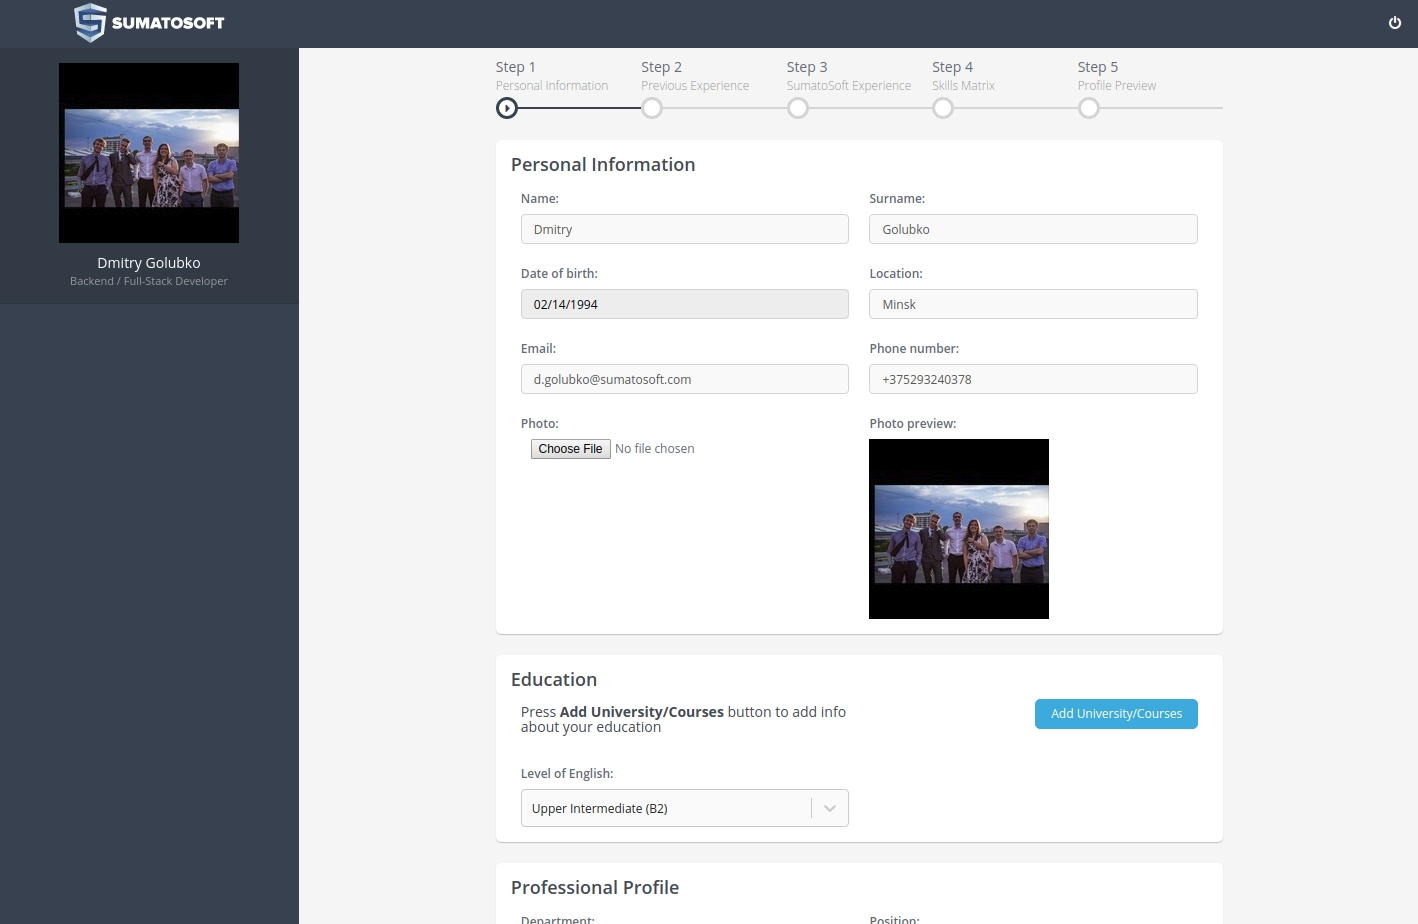
\includegraphics[scale=0.44]{agenda_screen.jpg}
    \caption{Экран заполнения профиля}
    \label{fig:manual:agenda_screen}
\end{figure}
  
Если авторизоваться в качестве администратора, то будет доступно меню функций, показанное на
рисунке~\ref{fig:manual:menu}

\begin{figure}[ht]
  \centering
    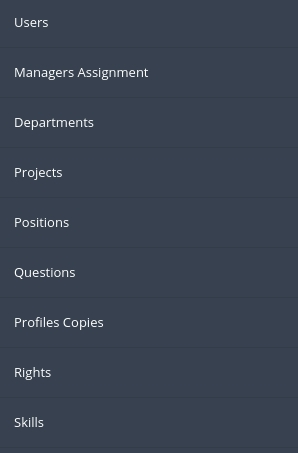
\includegraphics[scale=1]{menu.jpg}
    \caption{Меню функций администратора}
    \label{fig:manual:menu}
\end{figure}
  
На рисунке~\ref{fig:manual:managers_assignment} представлена страница назначения менеджеров. Страница выполнена в виде
таблицы, где строками являются департаменты, а столбцами - тип менеджера. Назначение менеджеров происходит путем выбора
из выпадающего списка пользователей для назачения в качестве соответствующего менеджера в соответствующем департаменте.

При открытии менеджером страницы профиля появляются функции, показанные на рисунке~\ref{fig:manual:profile_functions}

\begin{figure}[ht]
  \centering
    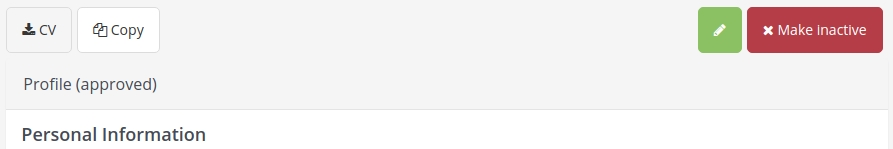
\includegraphics[scale=0.7]{profile_functions.jpg}
    \caption{Функции с профилем, доступные администратору}
    \label{fig:manual:profile_functions}
\end{figure}

\pagebreak

Назначение функций профиля следующее:
\begin{itemize}
	\item кнопка <<СV>> - кнопка генерации резюме, генерирует из профиля резюме в формате pdf;
  \item кнопка <<Copy>> - кнопка создания копии профиля, позволяет делать копии профиля для дальнейшего редактирования
  и создания резюме без изменения основного профиля. Все копии профилей находятся в отдельном меню, доступ к ним имеют
  только менеджеры, их редактирование никак не влияет на основной профиль;
	\item кнопка <<Редактировать>> - кнопка, открывающая профиль для редактирования;
	\item кнопка <<Make Inactive>> - кнопка, деактивирующая профиль.
\end{itemize}

\begin{figure}[ht]
  \centering
    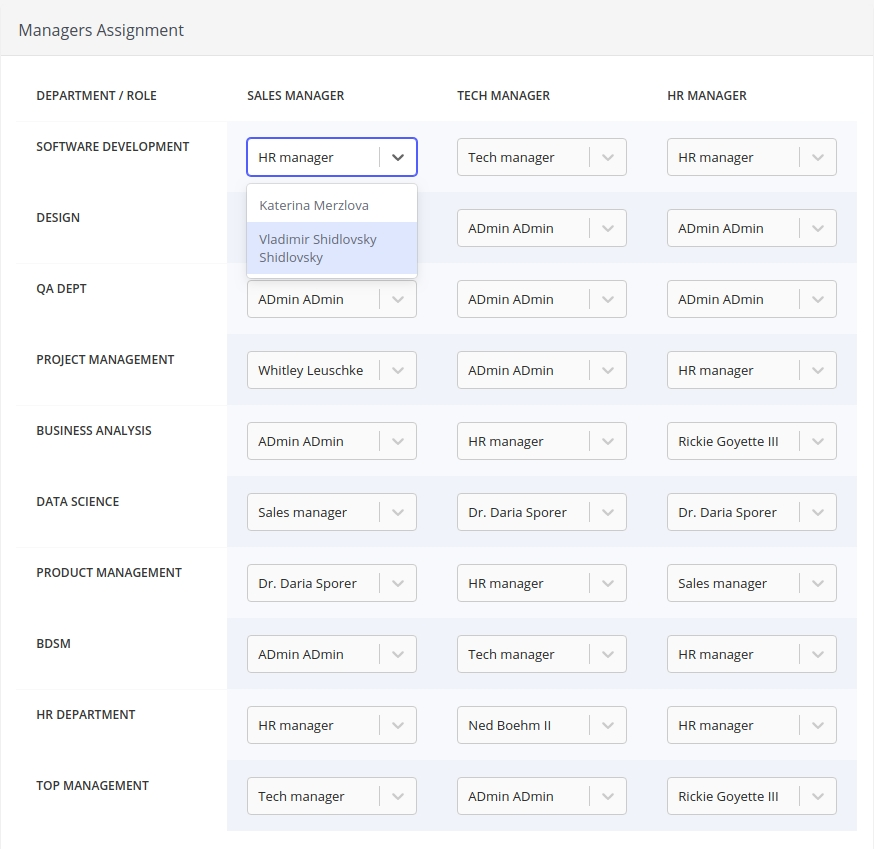
\includegraphics[scale=0.7]{managers_assignment.jpg}
    \caption{Страница назначения менеджеров}
    \label{fig:manual:managers_assignment}
\end{figure}

Сгенерированное из профиля резюме представлено на рисунке~\ref{fig:manual:resume}

\begin{sidewaysfigure}
  \centering
    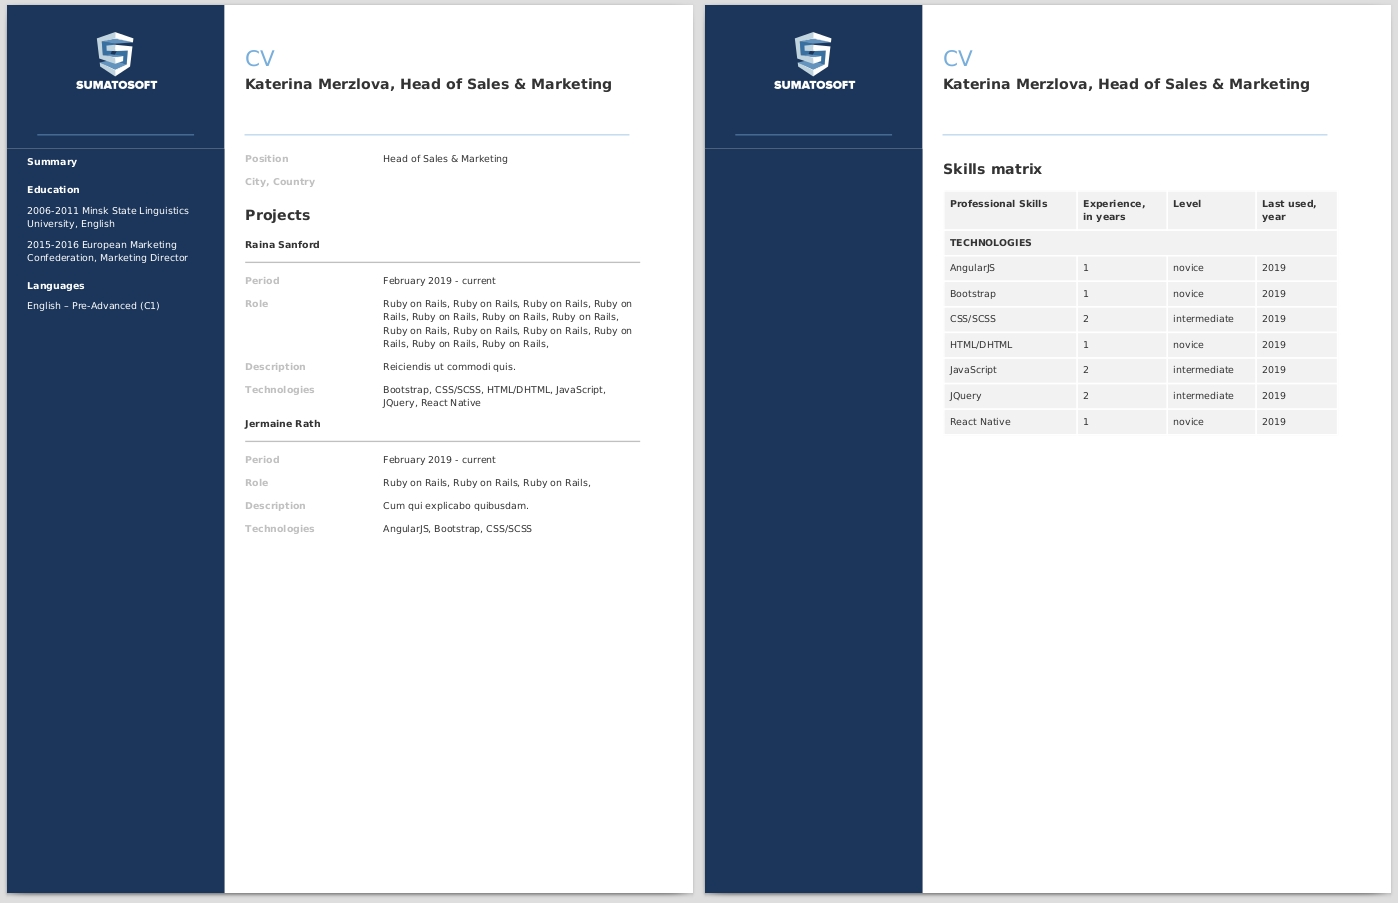
\includegraphics[scale=0.7]{resume.jpg}
    \caption{Страница назначения менеджеров}
    \label{fig:manual:resume}
\end{sidewaysfigure}
